\chapter{Análisis}

En esta sección se estudian las capacidades básicas que debe tener un producto mínimo viable de la aplicación, así como los actores que interactúan con el sistema y, los casos de uso y diagramas de secuencia más importantes. Finalmente, se describe el diagrama entidad relación de la base de datos.

\section{Requisitos Funcionales}

En esta sección se recopilan los requisitos funcionales más importantes que cumple el producto mínimo viable de la aplicación. Los requisitos funcionales son aquellos que definen los comportamientos, acciones y servicios que el sistema debe proporcionar al usuario. 

En \textit{Booster} los requisitos funcionales se recopilan a continuación separados por distintos bloques. 

\subsection{Gestión de usuario}

\begin{enumerate}[label=\textbf{RF-GU \arabic*.}, leftmargin=*]
    \item El sistema debe permitir a los usuarios registrarse en la plataforma con un correo o nombre de usuario.
    \item El sistema debe enviar un código de verificación al correo proporcionado para completar el registro o, luego de un tiempo de inactividad de un usuario registrado. 
    \item El sistema debe permitir a los usuarios iniciar sesión con un correo o nombre de usuario.
    \item El sistema debe permitir a los usuarios cerrar sesión
    \item El sistema debe permitir a los usuarios recuperar su contraseña.
    \item El sistema debe permitir al usuario subir una foto de perfil. 
    \item El sistema debe permitir a los usuarios editar foto de perfil, nombre, nombre de usuario y correo electrónico.
    \item El sistema debe permitir al usuario registrarse e iniciar sesión con una cuenta de Google.

\end{enumerate}

\subsection{Carga, gestión y moderación de videos}



\begin{enumerate}[label=\textbf{RF-CGMV \arabic*.}, leftmargin=*]
    \item El sistema debe permitir al usuario cargar un video a la plataforma.
    \item El sistema debe permitir al usuario agregar título, descripción y categoría al video.
    \item El sistema debe permitir al usuario seleccionar la visibilidad del video.
    \item El sistema debe permitir al usuario asociar un video a una comunidad.
    \item El sistema debe permitir al usuario eliminar un video propio.
    \item El sistema debe almacenar la información del video y sus metadatos.
    \item El sistema debe implementar un Adaptive Bitrate Streaming para la reproducción de video, lo que implica generar versiones de diferentes calidades.
    \item El sistema debe permitir al usuario reportar un video.
    \item El sistema debe permitir al usuario participar en votaciones para decidir si un video infringe las normas o no.
\end{enumerate}

\subsection{Reproducción y consumo de contenido}



\begin{enumerate}[label=\textbf{RF-RCC \arabic*.}, leftmargin=*]
    \item El sistema debe permitir al usuario visualizar un video.
    \item El sistema debe permitir al usuario pausar, reanudar, adelantar y retroceder el video.
    \item El sistema debe permitir al usuario cambiar la calidad de reproducción cuando existan varias resoluciones disponibles.
    \item El sistema debe permitir al usuario reproducir videos en pantalla completa.
    \item El sistema debe registrar visualizaciones del video.
    \item El sistema debe permitir al usuario navegar al siguiente video desde la interfaz de visualización.
    \item El sistema debe recomendar al usuario videos relacionados.
    \item El sistema debe mostrar información del video, como título, descripción, número de visualizaciones, fecha de publicación, descripción y creador.
\end{enumerate}

\subsection{Exploración y búsqueda}

\begin{enumerate}[label=\textbf{RF-EB \arabic*.}, leftmargin=*]
    \item El sistema debe permitir al usuario buscar videos por título, descripción o creador.
    \item El sistema debe permitir al usuario filtrar videos por categorías.
    \item El sistema debe recomendar al usuario videos en una cuadrícula principal.
    \item El sistema debe permitir al usuario visualizar contenido reciente de comunidades y creadores que sigue.
    \item El sistema debe permitir al usuario filtrar videos hechos por inteligencia artificial o con formato vertical. 
    \item El sistema debe permitir al usuario explorar comunidades y ver su contenido reciente.
\end{enumerate}

\subsection{Interacción social}
\begin{enumerate}[label=\textbf{RF-IS \arabic*.}, leftmargin=*]
    \item El sistema debe permitir al usuario calificar un video en una escala de 1 a 5 estrellas.
    \item El sistema debe permitir al usuario comentar en un video.
    \item El sistema debe permitir al usuario responder a un comentario existente.
    \item El sistema debe permitir al usuario editar o eliminar sus propios comentarios.
    \item El sistema debe mostrar los comentarios en estructura jerárquica o en árbol.
    \item El sistema debe recomendar los comentarios más relevantes o populares primero.
    \item El sistema debe permitir a un usuario donar puntos de experiencia a un canal. 
\end{enumerate}

\subsection{Comunidades}

\begin{enumerate}[label=\textbf{RF-COM \arabic*.}, leftmargin=*]
    \item El sistema debe permitir al usuario crear una comunidad.
    \item El sistema debe permitir al usuario unirse a comunidades.
    \item El sistema debe permitir al usuario abandonar comunidades.
    \item El sistema debe permitir al usuario consultar las comunidades a las que pertenece.
    \item El sistema debe permitir al usuario consultar los videos más recientes asociados a una comunidad.
    \item El sistema debe permitir al usuario buscar comunidades por nombre o descripción.
    \item El sistema debe permitir al usuario filtrar comunidades por categorías.
\end{enumerate}

\subsection{Canales}

\begin{enumerate}[label=\textbf{RF-CAN \arabic*.}, leftmargin=*]
    \item El sistema debe permitir al usuario gestionar y personalizar su canal.
    \item El sistema debe permitir al usuario visualizar la pestaña de videos de un canal.
    \item El sistema debe permitir al usuario visualizar la pestaña ranking de canal con la clasificación de los usuario donantes.
    \item El sistema debe permitir al usuario acceder a la pestaña de recompensas desbloqueadas de un canal.
    \item El sistema debe permitir al usuario visualizar la pestaña de información o descripción del canal.
    \item El sistema debe permitir al usuario acceder al chat comunitario de un canal o comunidad.
    \item El sistema debe permitir al usuario consultar su propio canal.
    \item El sistema debe permitir al usuario seguir a otros canales.
    \item El sistema debe permitir al usuario dejar de seguir a otros canales.
    \item El sistema debe permitir al usuario consultar los canales que sigue.
\end{enumerate}


\subsection{Gamificación}

\begin{enumerate}[label=\textbf{RF-GAM \arabic*.}, leftmargin=*]
    \item El sistema debe tener un recuento de los puntos de experiencia (XP) de cada usuario.
    \item El sistema debe permitir al usuario ganar puntos de experiencia al mirar anuncios.
    \item El sistema debe permitir al usuario consultar los puntos de boost y el nivel de un canal.
    \item El sistema debe mostrar una clasificación de los canales más populares según el número de seguidores y el nivel de canal.
    \item El sistema debe permitir al usuario visualizar artículos, recompensas o personalizaciones disponibles en la tienda.
    \item El sistema debe permitir al usuario comprar artículos de personalización en la tienda con puntos de experiencia. 
    \item El sistema debe permitir al usuario visualizar su inventario de artículos adquiridos.
    \item El sistema debe mostrar badges o iconos especiales en el perfil del usuario.
    \item El sistema debe reflejar visualmente los cambios de nivel recientes.
\end{enumerate}

\section{Requisitos No Funcionales}

Los requisitos no funcionales son aquellos que definen cómo debe comportarse el sistema en términos de rendimientos, seguridad, usabilidad, escalabilidad, en lugar de qué acciones se deben realizar.

\begin{enumerate}[label=\textbf{RNF \arabic*.}, leftmargin=*]
    \item \textbf{Rendimiento: } El sistema debe ser capaz de cargar las páginas en un tiempo aceptable (menos de 3 segundos) y reproducir videos sin interrupciones o buffering excesivo.
    \item \textbf{Seguridad:} El sistema debe proteger la información de los usuarios. Se deben implementar medidas de seguridad frente a ataques comunes como inyección SQL y prevenir el uso abusivo de la plataforma mediante la implementación de \textit{rate limits}.
    \item \textbf{Usabilidad:} El sistema debe tener una interfaz intuitiva y fácil de usar. 
    \item \textbf{Disponibilidad:} El sistema debe estar activo la mayor cantidad de tiempo posible, minimizando el tiempo de inactividad.
    \item \textbf{Escalabilidad: } El sistema debe ser capaz de manejar un aumento en el número de usuarios, interacciones y contenido sin degradar el rendimiento.
    \item \textbf{Compatibilidad: } El sistema debe funcionar correctamente en diferentes navegadores web y dispositivos. Esto incluye, navegadores populares como Chrome, Firefox, Safari y Edge, así como dispositivos móviles y de escritorio.
    \item \textbf{Mantenibilidad: } El sistema debe estar diseñado con patrones claros, utilizando buenas prácticas de desarrollo para facilitar su mantenimiento y evolución.
    \item \textbf{Modularidad: } El sistema debe estar diseñado de tal forma que sus componentes sean independientes y puedan evolucionar o ser reemplazados sin afectar al resto del sistema. 
\end{enumerate}

\section{Actores}

En un sistema software, los actores son entidades externas que interactúan con el sistema. Pueden ser usuarios humanos, otros sistemas o dispositivos. En el caso de \textit{Booster}, los actores principales son:

\begin{itemize}
    \item \textbf{Usuario visitante: } Un usuario que accede a la plataforma sin iniciar sesión. Este, puede explorar, buscar y consumir contenido, acceder a canales, acceder a los rankings, pero no puede interactuar con el sistema ni guardad sus preferencias.
    \item \textbf{Usuario registrado: } Un usuario que ha creado una cuenta e iniciado sesión en la plataforma. Este, además de las capacidades de un usuario visitante, puede cargar videos, interactuar con el contenido, participar en comunidades, seguir canales, personalizar su experiencia y ganar puntos de experiencia.
    \item \textbf{Creador de contenido: } Un usuario registrado que se dedica a crear videos en la plataforma. Además de consumir, puede gestionar su contenido y canal.   
    % \item \textbf{Sistema de backend: } Es el encargado de gestionar la lógica de negocio, el almacenamiento de datos, la autenticación, el recuento de puntos, el algoritmo de recomendación, entre otras funciones. Interactúa con los usuarios a través de la interfaz (\textit{frontend}).
    \item \textbf{Sistema de procesamiento de videos: } Es el encargado de procesar los videos cargados por un usuario. Cuando un video es subido, este se encarga de la transcodificación, la implementación de Adaptive Bitrate Streaming, generación de miniaturas, para servir los videos.    
\end{itemize}

\section{Casos de uso}

Un caso de uso es una descripción de cómo un actor interactúa con el sistema para alcanzar un objetivo. A continuación se muestran los diagramas de caso de uso más importantes detectados y, posteriormente, una descripción de cada uno de ellos.

\subsection{Gestión de usuarios}

Los casos de uso relacionados con la gestión de usuario son:

\begin{enumerate}
    \item Registro de usuario
    \item Iniciar sesión
    \item Recuperar contraseña
    \item Cerrar sesión 
    \item Gestionar perfil de usuario
\end{enumerate}
\clearpage

\textbf{Diagrama}

\begin{figure}[H]
  \centering
  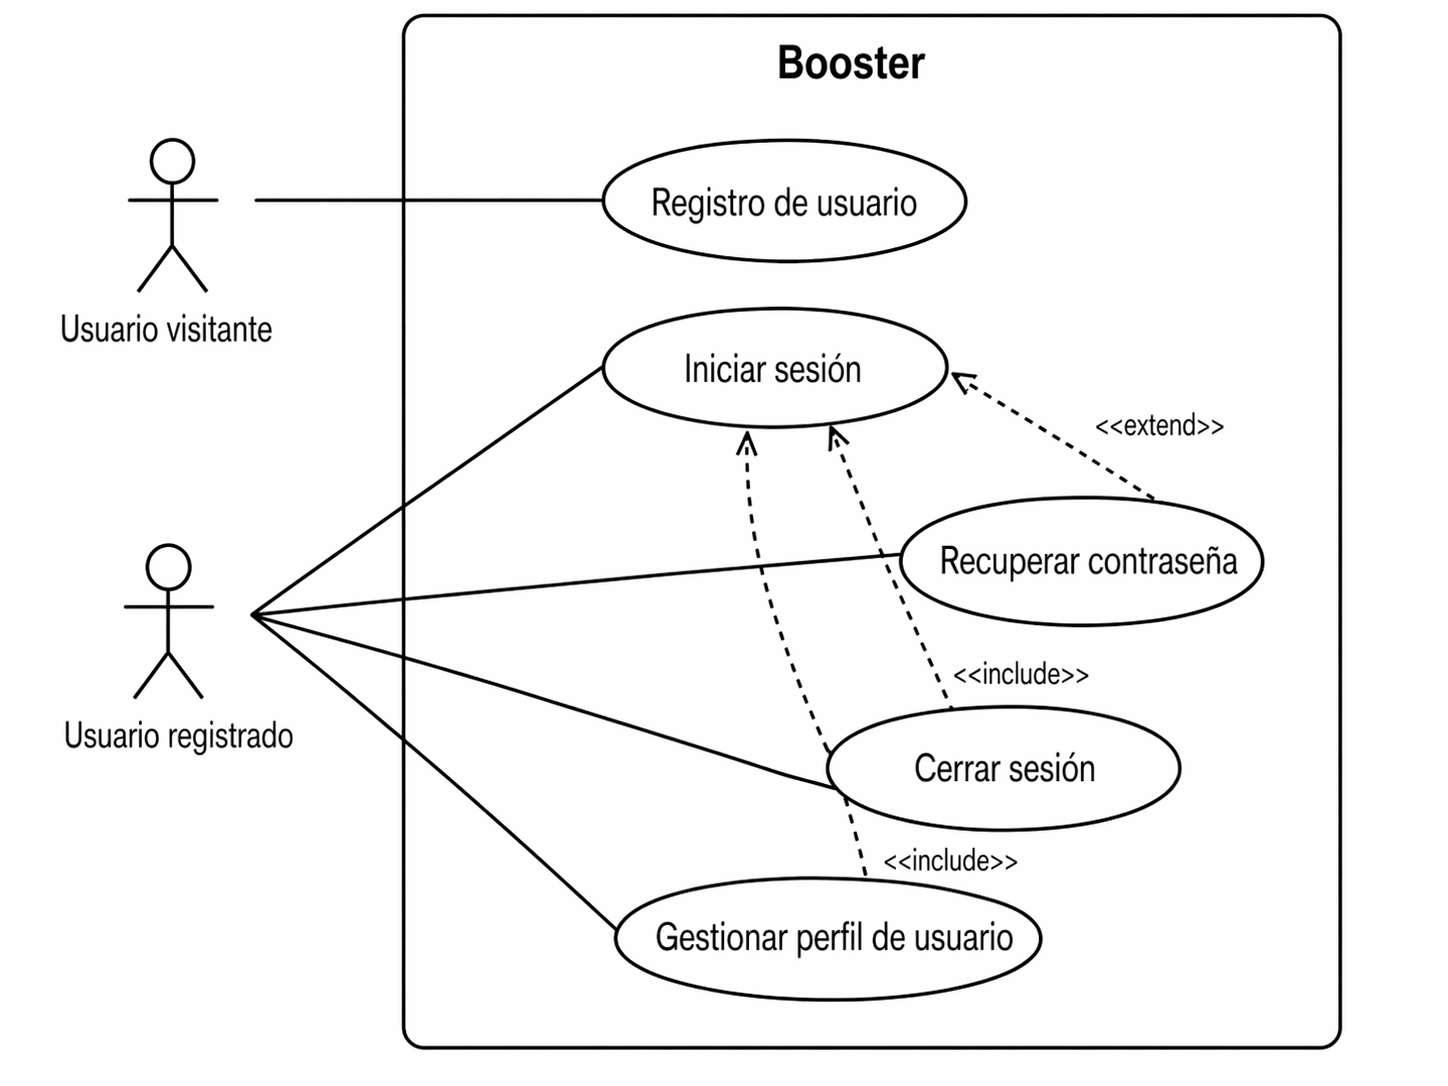
\includegraphics[width=0.8\textwidth]{casos-uso/iniciar-sesion.png}
  \caption{Gestión de usuarios en la plataforma - Casos de uso}
\end{figure}


\textbf{Descripción}

%TABLA REGISTRO
\begin{longtable}{|p{0.28\textwidth}|p{0.64\textwidth}|}
\hline
\rowcolor[gray]{0.75}
\multicolumn{2}{|c|}{\textbf{Caso de uso: Registro de usuario}} \\
\hline
\textbf{Actores} & Usuario visitante \\
\hline
\textbf{Descripción} & Permite a un usuario crear una cuenta nueva en la plataforma mediante correo electrónico, nombre de usuario y contraseña. También es posible utilizar una cuenta de Google. \\
\hline
\textbf{Precondiciones} & El usuario no ha iniciado sesión y accede a la pantalla de registro. \\
\hline
\textbf{Flujo principal} &
\begin{enumerate}
    \item  El usuario accede al formulario de registro. 
    \item  El sistema solicita los datos necesarios para crear la cuenta. 
    \item  El usuario introduce un correo electrónico, nombre de usuario y contraseña. 
    \item  El sistema valida la información introducida. 
    \item  El sistema envía un código de verificación al correo proporcionado. 
    \item  El usuario introduce el código de verificación recibido. 
    \item  El sistema verifica el código introducido. 
    \item  El sistema crea la cuenta de usuario. 
    \item  El sistema confirma que el registro se ha realizado correctamente. 
    \item  El sistema redirige al usuario a la pantalla de inicio de sesión. 
\end{enumerate} \\ 
\hline



\rowcolor[gray]{0.75}
\multicolumn{2}{|c|}{\textbf{Flujo alternativo al paso 3: registro con Google}} \\
\hline
\multicolumn{2}{|p{0.92\textwidth}|}{

\begin{enumerate}[label=3\alph*.]
    \item El usuario selecciona la opción de registro con Google. 
    \item El sistema redirige al proveedor de autenticación de Google (OAuth) para completar el proceso.
    \item Si el proceso falla o es cancelado, el sistema muestra un mensaje de error y regresa a la pantalla de registro.
    \item  Si la autenticación es correcta, el sistema crea la cuenta del usuario con los datos recibidos.
    \item El sistema confirma el registro exitoso y redirige al usuario a la pantalla principal.
\end{enumerate}
} \\
\hline


\rowcolor[gray]{0.75}
\multicolumn{2}{|c|}{\textbf{Flujo alternativo al paso 4: datos inválidos o inseguros}} \\
\hline
\multicolumn{2}{|p{0.92\textwidth}|}{

\begin{enumerate}[label=4\alph*.]
    \item Si los datos introducidos no cumplen las reglas de validación, como contraseñas débiles, el sistema muestra los errores correspondientes en el formulario. 
    \item El usuario corrige los errores señalados. 
    \item El sistema vuelve a validar la información introducida.
\end{enumerate} 
} \\
\hline

\rowcolor[gray]{0.75}
\multicolumn{2}{|c|}{\textbf{Flujo alternativo al paso 4: correo o nombre de usuario existente}} \\
\hline

\multicolumn{2}{|p{0.92\textwidth}|}{
    \begin{enumerate}[label=4\alph*.]
    \item Si el correo electrónico o el nombre de usuario ya existe, el sistema informa del conflicto y solicita datos diferentes. 
    \item El usuario introduce un correo o nombre de usuario distinto. 
    \item El sistema vuelve a validar la información introducida.
\end{enumerate}

} \\
\hline

\rowcolor[gray]{0.75}
\multicolumn{2}{|c|}{\textbf{Flujo alternativo al paso 7: código incorrecto o expirado}} \\
\hline
\multicolumn{2}{|p{0.92\textwidth}|}{

\begin{enumerate}[label=7\alph*.]
    \item Si el código introducido es incorrecto o ha expirado, el sistema muestra un mensaje de error y solicita un nuevo intento.
    \item El usuario introduce nuevamente el código de verificación recibido. 
    \item El sistema vuelve a verificar el código.
\end{enumerate}

} \\
\hline


\textbf{Postcondiciones} & La cuenta del usuario se crea y se almacena en la base de datos. \\
\hline
\textbf{Requisitos relacionados} & RF-GU 1, RF-GU 2, RF-GU 8 \\
\hline
\end{longtable}









%TABLA INICIAR SESION
\begin{longtable}{|p{0.28\textwidth}|p{0.64\textwidth}|}
\hline
\rowcolor[gray]{0.75}
\multicolumn{2}{|c|}{\textbf{Caso de uso: Iniciar sesión}} \\
\hline
\textbf{Actores} & Usuario registrado \\
\hline
\textbf{Descripción} & Permite a un usuario autenticarse en la plataforma mediante correo electrónico o nombre de usuario y contraseña. También es posible iniciar sesión con una cuenta de Google. \\
\hline
\textbf{Precondiciones} & El usuario dispone de una cuenta y no ha iniciado sesión. \\
\hline
\textbf{Flujo principal} &
\begin{enumerate}
    \item El usuario accede a la pantalla de inicio de sesión.
    \item El sistema solicita las credenciales.
    \item El usuario introduce su correo electrónico o nombre de usuario y contraseña.
    \item El sistema valida las credenciales.
    \item El sistema autentica al usuario.
    \item El sistema inicia la sesión y redirige al usuario a la pantalla principal.
\end{enumerate} \\
\hline

\rowcolor[gray]{0.75}
\multicolumn{2}{|c|}{\textbf{Flujo alternativo al paso 3: inicio de sesión con Google}} \\
\hline
\multicolumn{2}{|p{0.92\textwidth}|}{
\begin{enumerate}[label=3\alph*.]
    \item El usuario selecciona la opción de iniciar sesión con Google.
    \item El sistema redirige al proveedor de autenticación de Google (OAuth) para completar el proceso.
    \item Si el proceso falla o es cancelado, el sistema muestra un mensaje de error y regresa a la pantalla de inicio de sesión.
    \item Si la autenticación es correcta, el sistema autentica al usuario.
    \item El sistema inicia la sesión y redirige al usuario a la pantalla principal.
\end{enumerate}
} \\
\hline

\rowcolor[gray]{0.75}
\multicolumn{2}{|c|}{\textbf{Flujo alternativo al paso 3: recuperar contraseña}} \\
\hline
\multicolumn{2}{|p{0.92\textwidth}|}{
\begin{enumerate}[label=3\alph*.]
    \item El usuario selecciona la opción de recuperar contraseña.
    \item El sistema redirige al usuario al caso de uso \textit{Recuperar contraseña}.
\end{enumerate}
} \\
\hline

\rowcolor[gray]{0.75}
\multicolumn{2}{|c|}{\textbf{Flujo alternativo al paso 4: credenciales incorrectas}} \\
\hline
\multicolumn{2}{|p{0.92\textwidth}|}{
\begin{enumerate}[label=4\alph*.]
    \item Si las credenciales introducidas no son correctas, el sistema muestra un mensaje de error.
    \item El sistema regresa a la pantalla de inicio de sesión y solicita un nuevo intento.
\end{enumerate}
} \\
\hline

\rowcolor[gray]{0.75}
\multicolumn{2}{|c|}{\textbf{Flujo alternativo al paso 4: verificación adicional por inactividad}} \\
\hline
\multicolumn{2}{|p{0.92\textwidth}|}{
\begin{enumerate}[label=4\alph*.]
    \item Si el sistema detecta un periodo prolongado de inactividad de la cuenta, envía un código de verificación al correo electrónico registrado.
    \item El usuario introduce el código de verificación recibido.
    \item El sistema valida el código introducido.
    \item Si el código es correcto, el flujo continúa en el paso 5 del Flujo principal.
\end{enumerate}
} \\
\hline

\rowcolor[gray]{0.75}
\multicolumn{2}{|c|}{\textbf{Flujo alternativo al paso 4a: código de verificación incorrecto o expirado}} \\
\hline
\multicolumn{2}{|p{0.92\textwidth}|}{
\begin{enumerate}[label=4a\roman*.]
    \item Si el código introducido es incorrecto o ha expirado, el sistema muestra un mensaje de error y solicita un nuevo intento.
    \item Se regresa al paso 4b.
\end{enumerate}
} \\
\hline

\textbf{Postcondiciones} & El usuario accede a la plataforma con una sesión activa. \\
\hline
\textbf{Requisitos relacionados} & RF-GU 2, RF-GU 3, RF-GU 8 \\
\hline
\end{longtable}







%TABLA Recuperar Contraseña

\begin{longtable}{|p{0.28\textwidth}|p{0.64\textwidth}|}
\hline
\rowcolor[gray]{0.75}
\multicolumn{2}{|c|}{\textbf{Caso de uso: Recuperar contraseña}} \\
\hline
\textbf{Actores} & Usuario registrado \\
\hline
\textbf{Descripción} & Permite a un usuario restablecer la contraseña de su cuenta. Para esto, el sistema envía un código o enlace de verificación al correo electrónico asociado. \\
\hline
\textbf{Precondiciones} & El usuario dispone de una cuenta previamente registrada y no ha iniciado sesión. \\
\hline
\textbf{Flujo principal} &
\begin{enumerate}
    \item El usuario accede a la opción de recuperar contraseña desde la pantalla de inicio de sesión.
    \item El sistema solicita el correo electrónico asociado a la cuenta.
    \item El usuario introduce su correo electrónico.
    \item El sistema valida que exista una cuenta asociada a ese correo.
    \item El sistema envía un código al correo electrónico registrado.
    \item El usuario introduce el código de verificación.
    \item El sistema valida el código.
    \item El sistema solicita al usuario una nueva contraseña y su confirmación.
    \item El usuario introduce la nueva contraseña y su confirmación.
    \item El sistema valida la nueva contraseña.
    \item El sistema actualiza la contraseña de la cuenta.
    \item El sistema confirma que el restablecimiento se ha realizado correctamente y redirige al usuario a la pantalla de inicio de sesión.
\end{enumerate} \\
\hline

\rowcolor[gray]{0.75}
\multicolumn{2}{|c|}{\textbf{Flujo alternativo al paso 4: correo no registrado}} \\
\hline
\multicolumn{2}{|p{0.92\textwidth}|}{
\begin{enumerate}[label=4\alph*.]
    \item Si el correo electrónico introducido no está asociado a ninguna cuenta, el sistema muestra un mensaje de error solicitando al usuario que introduzca un correo válido y registrado.
\end{enumerate}
} \\
\hline

\rowcolor[gray]{0.75}
\multicolumn{2}{|c|}{\textbf{Flujo alternativo al paso 7: código inválido}} \\
\hline
\multicolumn{2}{|p{0.92\textwidth}|}{
\begin{enumerate}[label=7\alph*.]
    \item Si el código introducido no es válido, el sistema muestra un mensaje de error.
    \item El sistema solicita un nuevo intento de verificación.
\end{enumerate}
} \\
\hline

\rowcolor[gray]{0.75}
\multicolumn{2}{|c|}{\textbf{Flujo alternativo al paso 7: código expirado}} \\
\hline
\multicolumn{2}{|p{0.92\textwidth}|}{
\begin{enumerate}[label=7\alph*.]
    \item Si el código introducido ha expirado, el sistema lo informa.
    \item El sistema solicita al usuario que reinicie el proceso de recuperación de contraseña.
\end{enumerate}
} \\
\hline

\rowcolor[gray]{0.75}
\multicolumn{2}{|c|}{\textbf{Flujo alternativo al paso 10: contraseña inválida}} \\
\hline
\multicolumn{2}{|p{0.92\textwidth}|}{
\begin{enumerate}[label=10\alph*.]
    \item Si la nueva contraseña no coincide con la confirmación o esta no cumple con las reglas de seguridad establecidas, el sistema muestra los errores correspondientes.
    \item El usuario introduce una nueva contraseña válida y su confirmación.
    \item El sistema vuelve a validar la contraseña introducida.
\end{enumerate}
} \\
\hline

\textbf{Postcondiciones} & La contraseña de la cuenta queda actualizada en la base de datos y el usuario puede volver a iniciar sesión con la nueva contraseña. \\
\hline
\textbf{Requisitos relacionados} & RF-GU-5 \\
\hline
\end{longtable}


%TABLA Cerrar Sesion
\begin{longtable}{|p{0.28\textwidth}|p{0.64\textwidth}|}
\hline
\rowcolor[gray]{0.75}
\multicolumn{2}{|c|}{\textbf{Caso de uso: Cerrar sesión}} \\
\hline
\textbf{Actores} & Usuario registrado \\
\hline
\textbf{Descripción} & Permite a un usuario finalizar su sesión de forma segura. \\
\hline
\textbf{Precondiciones} & El usuario ha iniciado sesión en la plataforma. \\
\hline
\textbf{Flujo principal} &
\begin{enumerate}
    \item El usuario accede a la opción de cerrar sesión.
    \item El sistema invalida la sesión activa del usuario.
    \item El sistema redirige al usuario a la pantalla principal.
\end{enumerate} \\
\hline

\rowcolor[gray]{0.75}
\multicolumn{2}{|c|}{\textbf{Flujo alternativo al paso 2: sesión expirada}} \\
\hline
\multicolumn{2}{|p{0.92\textwidth}|}{
\begin{enumerate}[label=2\alph*.]
    \item Si la sesión del usuario ya ha expirado, el sistema informa de que no existe una sesión activa válida.
    \item El sistema redirige igualmente al usuario a la pantalla principal.
\end{enumerate}
} \\
\hline

\textbf{Postcondiciones} & La sesión del usuario queda finalizada y este deja de estar autenticado en la plataforma. \\
\hline
\textbf{Requisitos relacionados} & RF-GU-4 \\
\hline
\end{longtable}


%TABLA Gestion perfil de usuario

\begin{longtable}{|p{0.28\textwidth}|p{0.64\textwidth}|}
\hline
\rowcolor[gray]{0.75}
\multicolumn{2}{|c|}{\textbf{Caso de uso: Gestionar perfil de usuario}} \\
\hline
\textbf{Actores} & Usuario registrado \\
\hline
\textbf{Descripción} & Permite a un usuario registrado consultar y modificar la información básica de su perfil. Esto incluye, cambiar la foto de perfil, su nombre, nombre de usuario y su correo electrónico. \\
\hline
\textbf{Precondiciones} & El usuario ha iniciado sesión en la plataforma. \\
\hline
\textbf{Flujo principal} &
\begin{enumerate}
    \item El usuario accede a su perfil en la barra de navegación.
    \item El usuario selecciona la opción de editar perfil  (\textit{Manage account}).
    \item El usuario modifica uno o varios de los siguientes datos: foto de perfil, nombre, nombre de usuario o correo electrónico.
    \item El sistema valida la información introducida.
    \item El sistema guarda los cambios realizados.
    \item El sistema confirma que la actualización del perfil se ha realizado correctamente.
\end{enumerate} \\
\hline

\rowcolor[gray]{0.75}
\multicolumn{2}{|c|}{\textbf{Flujo alternativo al paso 4: datos inválidos}} \\
\hline
\multicolumn{2}{|p{0.92\textwidth}|}{
\begin{enumerate}[label=4\alph*.]
    \item Si alguno de los datos introducidos no cumple las reglas de validación, el sistema muestra los errores correspondientes.
    \item El usuario corrige los errores señalados.
    \item El sistema vuelve a validar la información.
\end{enumerate}
} \\
\hline

\rowcolor[gray]{0.75}
\multicolumn{2}{|c|}{\textbf{Flujo alternativo al paso 4: correo o nombre de usuario ya existente}} \\
\hline
\multicolumn{2}{|p{0.92\textwidth}|}{
\begin{enumerate}[label=4\alph*.]
    \item Si el nuevo correo electrónico o nombre de usuario ya está asociado a otra cuenta, el sistema informa del conflicto.
    \item El usuario introduce un correo electrónico o nombre de usuario diferente.
    \item El sistema vuelve a validar la información.
\end{enumerate}
} \\
\hline

\rowcolor[gray]{0.75}
\multicolumn{2}{|c|}{\textbf{Flujo alternativo al paso 4: error al subir la foto de perfil}} \\
\hline
\multicolumn{2}{|p{0.92\textwidth}|}{
\begin{enumerate}[label=4\alph*.]
    \item Si la imagen seleccionada no cumple el formato o tamaño permitido, el sistema muestra un mensaje de error. (Tamaño recomendado 1:1; Límite de peso es $10$MB.) 
    \item El usuario selecciona una imagen válida.
    \item El sistema permite continuar con la edición del perfil.
\end{enumerate}
} \\
\hline

\textbf{Postcondiciones} & La información actualizada del perfil queda almacenada en la base de datos del sistema. \\
\hline
\textbf{Requisitos relacionados} & RF-GU 6, RF-GU 7 \\
\hline
\end{longtable}



\subsection{Carga, gestión y moderación de videos}

Los casos de uso identificados relacionados con la carga, gestión y moderación de videos son:

\begin{enumerate}
    \item Subir video
    \item Editar metadatos del video
    \item Eliminar video
    \item Reportar video
    \item Votar en moderación de contenido
    \item Procesar video
\end{enumerate}

\clearpage

\textbf{Diagrama}

\begin{figure}[H]
  \centering
  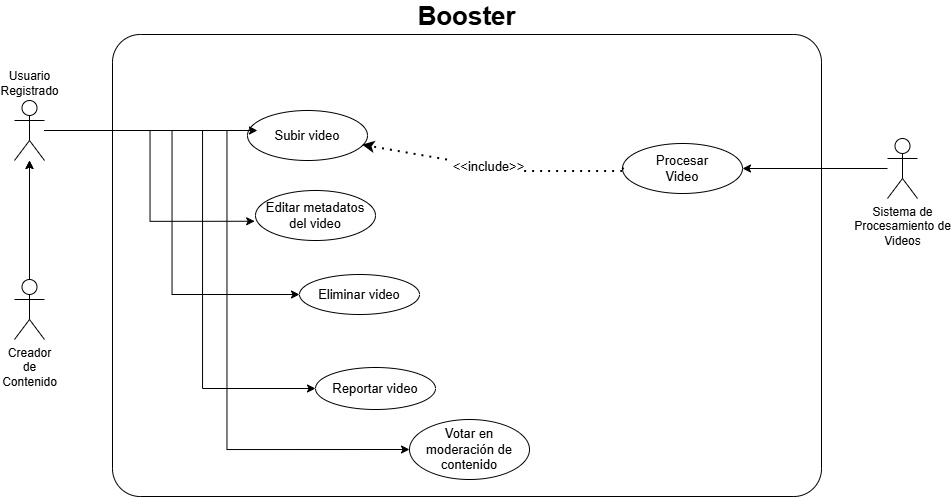
\includegraphics[width=1\textwidth]{casos-uso/subir-video.png}
  \caption{Carga de Videos a la plataforma - Casos de uso}
\end{figure}


\textbf{Descripción}


%SUBIR VIDEO

\begin{longtable}{|p{0.28\textwidth}|p{0.64\textwidth}|}
\hline
\rowcolor[gray]{0.75}
\multicolumn{2}{|c|}{\textbf{Caso de uso: Subir video}} \\
\hline
\textbf{Actores} & Usuario registrado, Creador de Contenido, Sistema de Procesamiento de Videos.\\
\hline
\textbf{Descripción} & Permite a un usuario registrado cargar un video a la plataforma, indicando sus datos básicos, su visibilidad y, opcionalmente, la comunidad a la que será asociado. \\
\hline
\textbf{Precondiciones} & El usuario ha iniciado sesión en la plataforma y dispone de un archivo de video válido. \\
\hline
\textbf{Flujo principal} &
\begin{enumerate}
    \item El usuario selecciona la opción de subir video.
    \item El sistema muestra el formulario de carga.
    \item El usuario selecciona el archivo de video que desea subir.
    \item El sistema recibe el archivo seleccionado y comienza a subirse al servidor.
    \item El usuario introduce el título, la descripción y la categoría del video.
    \item El usuario selecciona la visibilidad del video.
    \item El usuario indica, opcionalmente, la comunidad a la que desea asociar el video.
    \item El sistema almacena el video y sus metadatos.
    \item El sistema registra el video en la plataforma e inicia su procesamiento.
    \item El sistema confirma que la carga se ha realizado correctamente.
\end{enumerate} \\
\hline

\rowcolor[gray]{0.75}
\multicolumn{2}{|c|}{\textbf{Flujo alternativo al paso 3: archivo inválido}} \\
\hline
\multicolumn{2}{|p{0.92\textwidth}|}{
\begin{enumerate}[label=3\alph*.]
    \item Si el archivo seleccionado no corresponde a un formato de video permitido, excede el tamaño soportado o el límite de tiempo (10 minutos), el sistema muestra un mensaje de error.
    \item El usuario selecciona un archivo válido.
    \item El sistema permite continuar con el proceso de carga.
\end{enumerate}
} \\
\hline

\rowcolor[gray]{0.75}
\multicolumn{2}{|c|}{\textbf{Flujo alternativo al paso 5: datos inválidos}} \\
\hline
\multicolumn{2}{|p{0.92\textwidth}|}{
\begin{enumerate}[label=5\alph*.]
    \item Si alguno de los metadatos introducidos no cumple las reglas de validación como un título con más de 100 caracteres, el sistema muestra los errores correspondientes.
    \item El usuario corrige la información.
    \item El sistema vuelve a validar los metadatos.
\end{enumerate}
} \\
\hline


\rowcolor[gray]{0.75}
\multicolumn{2}{|c|}{\textbf{Flujo alternativo al paso 7: comunidad no válida}} \\
\hline
\multicolumn{2}{|p{0.92\textwidth}|}{
\begin{enumerate}[label=7\alph*.]
    \item Si la comunidad seleccionada no existe o el usuario no tiene permisos para publicar en ella, se muestra un mensaje de error.
    \item El usuario selecciona otra comunidad o decide no asociar el video a ninguna.
    \item El sistema continúa con el proceso de publicación.
\end{enumerate}
} \\
\hline

\textbf{Postcondiciones} & El video y sus metadatos quedan almacenados en el sistema y el procesamiento del contenido queda iniciado. \\
\hline
\textbf{Requisitos relacionados} & RF-CGMV 1, RF-CGMV 2, RF-CGMV 3, RF-CGMV 4, RF-CGMV 6 \\
\hline
\end{longtable}


%EDITAR METADATOS 

\begin{longtable}{|p{0.28\textwidth}|p{0.64\textwidth}|}
\hline
\rowcolor[gray]{0.75}
\multicolumn{2}{|c|}{\textbf{Caso de uso: Editar metadatos del video}} \\
\hline
\textbf{Actores} & Usuario registrado o Creador de Contenido \\
\hline
\textbf{Descripción} & Permite al propietario de un video modificar su título, descripción, categoría, visibilidad y comunidad asociada. \\
\hline
\textbf{Precondiciones} & El usuario ha iniciado sesión en la plataforma y es el creador del video que desea editar. \\
\hline
\textbf{Flujo principal} &
\begin{enumerate}
    \item El usuario accede a la sección de gestión de sus videos (\textit{studio}).
    \item El sistema muestra la lista de videos del usuario.
    \item El usuario selecciona el video que desea editar.
    \item El sistema muestra los metadatos del video.
    \item El usuario modifica uno o varios de los siguientes datos: título, descripción, categoría, visibilidad o comunidad asociada.
    \item El sistema valida la información introducida.
    \item El usuario guarda los cambios.
    \item El sistema actualiza la información del video.
    \item El sistema confirma que la edición se ha realizado correctamente.
\end{enumerate} \\
\hline

\rowcolor[gray]{0.75}
\multicolumn{2}{|c|}{\textbf{Flujo alternativo al paso 3: video no editable}} \\
\hline
\multicolumn{2}{|p{0.92\textwidth}|}{
\begin{enumerate}[label=3\alph*.]
    \item Si el video no existe o no pertenece al usuario, el sistema muestra un mensaje de error.
    \item El sistema impide continuar con la edición y regresa a la lista de videos.
\end{enumerate}
} \\
\hline

\rowcolor[gray]{0.75}
\multicolumn{2}{|c|}{\textbf{Flujo alternativo al paso 6: datos inválidos}} \\
\hline
\multicolumn{2}{|p{0.92\textwidth}|}{
\begin{enumerate}[label=6\alph*.]
    \item Si alguno de los metadatos introducidos no cumple las reglas de validación, el sistema muestra los errores correspondientes.
    \item El usuario corrige la información.
    \item El sistema vuelve a validar los metadatos.
\end{enumerate}
} \\
\hline

\rowcolor[gray]{0.75}
\multicolumn{2}{|c|}{\textbf{Flujo alternativo al paso 5: comunidad no válida}} \\
\hline
\multicolumn{2}{|p{0.92\textwidth}|}{
\begin{enumerate}[label=5\alph*.]
    \item Si la comunidad seleccionada no existe o el usuario no tiene permisos para publicar en ella, se muestra un mensaje de error..
    \item El usuario selecciona otra comunidad o elimina la asociación.
    \item El sistema permite continuar con la edición.
\end{enumerate}
} \\
\hline

\textbf{Postcondiciones} & Los metadatos actualizados del video quedan almacenados en el sistema. \\
\hline
\textbf{Requisitos relacionados} & RF-CGMV 2, RF-CGMV 3, RF-CGMV 4, RF-CGMV 6 \\
\hline
\end{longtable}

% ELIMINAR VIDEO

\begin{longtable}{|p{0.28\textwidth}|p{0.64\textwidth}|}
\hline
\rowcolor[gray]{0.75}
\multicolumn{2}{|c|}{\textbf{Caso de uso: Eliminar video}} \\
\hline
\textbf{Actores} & Usuario registrado o Creador de Contenido \\
\hline
\textbf{Descripción} & Permite al propietario de un video eliminarlo de la plataforma. \\
\hline
\textbf{Precondiciones} & El usuario ha iniciado sesión en la plataforma y es el creador del video que desea eliminar. \\
\hline
\textbf{Curso principal} &
\begin{enumerate}
    \item El usuario accede a la sección de gestión de sus videos.
    \item El sistema muestra la lista de videos del usuario.
    \item El usuario selecciona la opción de eliminar en el video deseado.
    \item El sistema solicita confirmación antes de proceder.
    \item El usuario confirma la eliminación.
    \item El sistema elimina el video de la plataforma y actualiza la base de datos.
    \item El sistema confirma que el video ha sido eliminado correctamente.
\end{enumerate} \\
\hline

\rowcolor[gray]{0.75}
\multicolumn{2}{|c|}{\textbf{Curso alternativo al paso 3: video no eliminable}} \\
\hline
\multicolumn{2}{|p{0.92\textwidth}|}{
\begin{enumerate}[label=3\alph*.]
    \item Si el video no existe o no pertenece al usuario, el sistema muestra un mensaje de error.
    \item El sistema impide la operación y regresa a la lista de videos.
\end{enumerate}
} \\
\hline

\rowcolor[gray]{0.75}
\multicolumn{2}{|c|}{\textbf{Curso alternativo al paso 4: cancelación de la eliminación}} \\
\hline
\multicolumn{2}{|p{0.92\textwidth}|}{
\begin{enumerate}[label=4\alph*.]
    \item El usuario decide no confirmar la eliminación.
    \item El sistema cancela la operación y no hay cambios.
\end{enumerate}
} \\
\hline

\textbf{Postcondiciones} & El video se elimina de la base de datos y deja de estar disponible en la plataforma. \\
\hline
\textbf{Requisitos relacionados} & RF-CGMV 5 \\
\hline
\end{longtable}


%REPORTAR VIDEO
\begin{longtable}{|p{0.28\textwidth}|p{0.64\textwidth}|}
\hline
\rowcolor[gray]{0.75}
\multicolumn{2}{|c|}{\textbf{Caso de uso: Reportar video}} \\
\hline
\textbf{Actores} & Usuario registrado \\
\hline
\textbf{Descripción} & Permite a un usuario registrado reportar un video por posible incumplimiento de las normas de la plataforma. \\
\hline
\textbf{Precondiciones} & El usuario ha iniciado sesión y accede a un video. \\
\hline
\textbf{Curso principal} &
\begin{enumerate}
    \item El usuario accede a un video de la plataforma.
    \item El usuario selecciona la opción de reportar video.
    \item El sistema muestra el formulario de reporte.
    \item El usuario selecciona el motivo del reporte y, opcionalmente, añade información adicional.
    \item El usuario confirma el envío del reporte.
    \item El sistema registra el reporte asociado al video y al usuario.
    \item El sistema confirma que el reporte ha sido enviado correctamente.
    \item El sistema abre una votación de moderación para ese video con el motivo seleccionado.
\end{enumerate} \\
\hline

\rowcolor[gray]{0.75}
\multicolumn{2}{|c|}{\textbf{Curso alternativo al paso 4: información incompleta}} \\
\hline
\multicolumn{2}{|p{0.92\textwidth}|}{
\begin{enumerate}[label=4\alph*.]
    \item Si el motivo del reporte no ha sido seleccionado o la información requerida está incompleta, el sistema muestra un mensaje de error.
    \item El usuario completa la información solicitada.
    \item El sistema permite continuar con el envío del reporte.
\end{enumerate}
} \\
\hline

\rowcolor[gray]{0.75}
\multicolumn{2}{|c|}{\textbf{Curso alternativo al paso 5: reporte duplicado}} \\
\hline
\multicolumn{2}{|p{0.92\textwidth}|}{
\begin{enumerate}[label=5\alph*.]
    \item Si el usuario ya había reportado previamente el video por el mismo motivo, el sistema informa de ello.
    \item El sistema impide registrar un nuevo reporte duplicado.
\end{enumerate}
} \\
\hline

\rowcolor[gray]{0.75}
\multicolumn{2}{|c|}{\textbf{Curso alternativo al paso 5: votación abierta}} \\
\hline
\multicolumn{2}{|p{0.92\textwidth}|}{
\begin{enumerate}[label=5\alph*.]
    \item Si el video había sido reportado por el mismo motivo, el sistema agrega un voto a favor en la votación de moderación y le indica al usuario que ya existía una votación abierta por el mismo motivo.
\end{enumerate}
} \\
\hline


\textbf{Postcondiciones} & El reporte del video queda almacenado en el sistema para su posterior revisión o votación. \\
\hline
\textbf{Requisitos relacionados} & RF-CGMV-8 \\
\hline
\end{longtable}


%MODERACION

\begin{longtable}{|p{0.28\textwidth}|p{0.64\textwidth}|}
\hline
\rowcolor[gray]{0.75}
\multicolumn{2}{|c|}{\textbf{Caso de uso: Votar en moderación de contenido}} \\
\hline
\textbf{Actores} & Usuario registrado \\
\hline
\textbf{Descripción} & Permite a un usuario registrado participar en una votación para decidir si un video reportado infringe o no las normas de la plataforma. \\
\hline
\textbf{Precondiciones} & El usuario ha iniciado sesión y existe una votación abierta sobre un video. \\
\hline
\textbf{Curso principal} &
\begin{enumerate}
    \item El usuario accede a un video.
    \item El sistema indica que existe una votación de moderación abierta para el  video en la sección de detalles del video.
    \item El usuario revisa el contenido reportado y las razones.
    \item El usuario emite su voto sobre si el video infringe o no las normas.
    \item El sistema registra el voto emitido.
    \item El sistema confirma que la votación se ha realizado correctamente.
\end{enumerate} \\
\hline

\rowcolor[gray]{0.75}
\multicolumn{2}{|c|}{\textbf{Curso alternativo al paso 2: no hay votaciones}} \\
\hline
\multicolumn{2}{|p{0.92\textwidth}|}{
\begin{enumerate}[label=2\alph*.]
    \item El sistema impide continuar con la acción de votar e indica que no hay votaciones disponibles.
\end{enumerate}
} \\
\hline

\rowcolor[gray]{0.75}
\multicolumn{2}{|c|}{\textbf{Curso alternativo al paso 4: voto ya emitido}} \\
\hline
\multicolumn{2}{|p{0.92\textwidth}|}{
\begin{enumerate}[label=4\alph*.]
    \item Si el usuario ya ha votado previamente sobre ese caso, el sistema informa de ello.
    \item El sistema impide registrar un nuevo voto para el mismo proceso de moderación.
\end{enumerate}
} \\
\hline

\textbf{Postcondiciones} & El voto del usuario queda almacenado en el sistema y asociado al proceso de moderación correspondiente. \\
\hline
\textbf{Requisitos relacionados} & RF-CGMV 9 \\
\hline
\end{longtable}



%PROCESAR VIDEO

\begin{longtable}{|p{0.28\textwidth}|p{0.64\textwidth}|}
\hline
\rowcolor[gray]{0.75}
\multicolumn{2}{|c|}{\textbf{Caso de uso: Procesar video}} \\
\hline
\textbf{Actores} & Sistema de procesamiento de videos \\
\hline
\textbf{Descripción} & Permite al sistema procesar automáticamente un video cargado, generando las copias necesarias para su reproducción en distintas calidades y \textit{bitrates} y almacenando los resultados asociados. \\
\hline
\textbf{Precondiciones} & Existe un video cargado en la plataforma pendiente de procesamiento. \\
\hline
\textbf{Curso principal} &
\begin{enumerate}
    \item El sistema registra que un nuevo video ha sido cargado.
    \item El sistema de procesamiento recibe el archivo del video. 
    \item El sistema de procesamiento analiza el archivo recibido.
    \item El sistema de procesamiento genera las distintas versiones de calidad del video.
    \item El sistema de procesamiento genera los recursos necesarios para implementar \textit{Adaptive Bitrate}.
    \item El sistema de procesamiento almacena los archivos procesados y le informa al sistema sobre los datos actualizados.
    \item El sistema marca el video como procesado y está disponible para su  reproducción en la plataforma.
\end{enumerate} \\
\hline

\rowcolor[gray]{0.75}
\multicolumn{2}{|c|}{\textbf{Curso alternativo al paso 3: archivo corrupto o no procesable}} \\
\hline
\multicolumn{2}{|p{0.92\textwidth}|}{
\begin{enumerate}[label=3\alph*.]
    \item Si el archivo se encuentra corrupto o no puede ser interpretado correctamente, el sistema de procesamiento registra el error y se lo informa al sistema.
    \item El sistema marca el video como fallido.
    \item El sistema notifica que el video no ha podido ser procesado.
\end{enumerate}
} \\
\hline

\rowcolor[gray]{0.75}
\multicolumn{2}{|c|}{\textbf{Curso alternativo al paso 4: fallo durante la transcodificación}} \\
\hline
\multicolumn{2}{|p{0.92\textwidth}|}{
\begin{enumerate}[label=4\alph*.]
    \item Si ocurre un error durante la generación de calidades, el sistema de procesamiento registra la incidencia.
    \item El sistema de procesamiento reintenta la operación.
    \item Si el error persiste, el sistema de procesamiento informa al sistema y el video queda marcado como no disponible.
\end{enumerate}
} \\
\hline

\textbf{Postcondiciones} & El video queda procesado y disponible para reproducción en la plataforma. \\
\hline
\textbf{Requisitos relacionados} & RF-CGMV 6, RF-CGMV 7 \\
\hline
\end{longtable}

\subsection{Reproducción y consumo de contenido}

Los casos de uso identificados relacionados con la reproducción y consumo de contenido son:

\begin{enumerate}
    \item Reproducir video
    \item Controlar ajustes de reproducción
    \item Información del video
    \item Videos relacionados
\end{enumerate}

\textbf{Diagrama}

\begin{figure}[H]
  \centering
  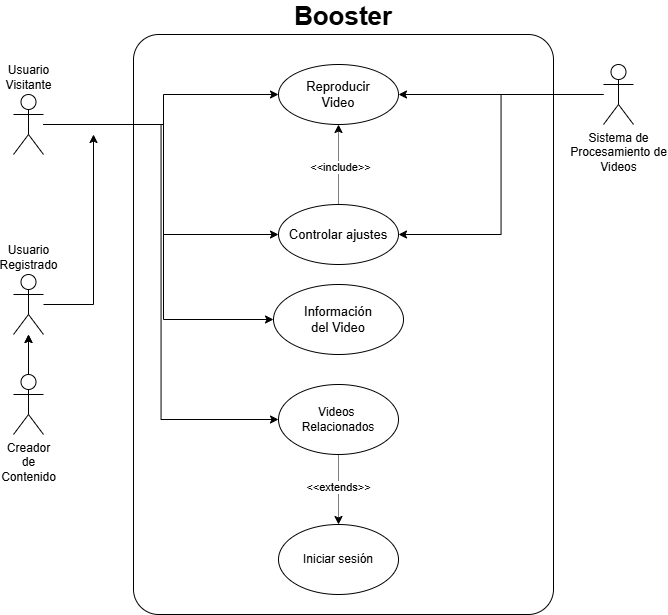
\includegraphics[width=1\textwidth]{casos-uso/reproduccion-consumo.png}
  \caption{Reproducción y consumo de contenido}
\end{figure}

\textbf{Descripción}


%REPRODUCIR VIDEO

\begin{longtable}{|p{0.28\textwidth}|p{0.64\textwidth}|}
\hline
\rowcolor[gray]{0.75}
\multicolumn{2}{|c|}{\textbf{Caso de uso: Reproducir video}} \\
\hline
\textbf{Actores} & Usuario visitante, Usuario registrado o Creador de Contenido y Sistema de procesamiento de videos \\
\hline
\textbf{Descripción} & Permite al usuario visualizar un video disponible en la plataforma. \\
\hline
\textbf{Precondiciones} & El video existe y está disponible para su visualización en la plataforma. \\
\hline
\textbf{Curso principal} &
\begin{enumerate}
    \item El usuario accede a un video desde la plataforma.
    \item El sistema carga el reproductor de video.
    \item El sistema le pide al sistema de procesamiento de videos los recursos.
    \item El sistema inicia la reproducción del video.
    \item El sistema registra la visualización del video.
    \item El usuario visualiza el contenido.
\end{enumerate} \\
\hline

\rowcolor[gray]{0.75}
\multicolumn{2}{|c|}{\textbf{Curso alternativo al paso 2: error de carga}} \\
\hline
\multicolumn{2}{|p{0.92\textwidth}|}{
\begin{enumerate}[label=2\alph*.]
    \item Si el reproductor no puede cargarse correctamente, el sistema muestra un mensaje de error.
    \item El sistema impide la reproducción del video.
\end{enumerate}
} \\
\hline

\textbf{Postcondiciones} & El video ha sido reproducido y su visualización queda registrada. \\
\hline
\textbf{Requisitos relacionados} & RF-RCC 1, RF-RCC 5 \\
\hline
\end{longtable}


%CONTROLAR AJUSTES 

\begin{longtable}{|p{0.28\textwidth}|p{0.64\textwidth}|}
\hline
\rowcolor[gray]{0.75}
\multicolumn{2}{|c|}{\textbf{Caso de uso: Controlar ajustes de reproducción}} \\
\hline
\textbf{Actores} & Usuario visitante, Usuario registrado o Creador de Contenido y Sistema de procesamiento de videos \\
\hline
\textbf{Descripción} & Permite al usuario controlar la reproducción del video mediante acciones como pausar, reanudar, adelantar, retroceder o cambiar la calidad. \\
\hline
\textbf{Precondiciones} & El video se encuentra en reproducción. \\
\hline
\textbf{Curso principal} &
\begin{enumerate}
    \item El usuario accede a los controles del reproductor.
    \item El usuario pausa o reanuda el video.
    \item El usuario adelanta o retrocede el video.
    \item El usuario cambia la calidad de reproducción si existen varias resoluciones disponibles y el sistema le pide al sistema de procesamiento de videos los recursos necesarios.
    \item El usuario activa o desactiva el modo de pantalla completa.
    \item El sistema aplica los cambios solicitados en tiempo real.
\end{enumerate} \\
\hline

\rowcolor[gray]{0.75}
\multicolumn{2}{|c|}{\textbf{Curso alternativo al paso 4: calidad no disponible}} \\
\hline
\multicolumn{2}{|p{0.92\textwidth}|}{
\begin{enumerate}[label=4\alph*.]
    \item Si la calidad seleccionada no está disponible, el sistema mantiene la calidad actual.
\end{enumerate}
} \\
\hline

\textbf{Postcondiciones} & El video se reproduce con los ajustes seleccionados por el usuario. \\
\hline
\textbf{Requisitos relacionados} & RF-RCC 2, RF-RCC 3, RF-RCC 4 \\
\hline
\end{longtable}

%INFORMACION DEL VIDEO

\begin{longtable}{|p{0.28\textwidth}|p{0.64\textwidth}|}
\hline
\rowcolor[gray]{0.75}
\multicolumn{2}{|c|}{\textbf{Caso de uso: Información del video}} \\
\hline
\textbf{Actores} & Usuario visitante, Usuario registrado o Creador de Contenido \\
\hline
\textbf{Descripción} & Permite al usuario consultar la información asociada a un video. \\
\hline
\textbf{Precondiciones} & El usuario accede a la interfaz de visualización de un video. \\
\hline
\textbf{Curso principal} &
\begin{enumerate}
    \item El usuario accede a la página de visualización de un video.
    \item El sistema muestra el título del video.
    \item El sistema muestra la descripción del video.
    \item El sistema muestra el número de visualizaciones.
    \item El sistema muestra la fecha de publicación.
    \item El sistema muestra el creador del contenido así como sus puntos de Boost y nivel.
\end{enumerate} \\
\hline

\textbf{Postcondiciones} & El usuario visualiza la información disponible del video. \\
\hline
\textbf{Requisitos relacionados} & RF-RCC 8 \\
\hline
\end{longtable}

%VIDEOS RELACIONADOS

\begin{longtable}{|p{0.28\textwidth}|p{0.64\textwidth}|}
\hline
\rowcolor[gray]{0.75}
\multicolumn{2}{|c|}{\textbf{Caso de uso: Videos relacionados}} \\
\hline
\textbf{Actores} & Usuario visitante, Usuario registrado \\
\hline
\textbf{Descripción} & Permite al usuario visualizar y acceder a videos recomendados relacionados con el contenido actual. \\
\hline
\textbf{Precondiciones} & El usuario se encuentra visualizando un video. \\
\hline
\textbf{Curso principal} &
\begin{enumerate}
    \item El usuario accede a la interfaz de visualización de un video.
    \item El sistema muestra una lista de videos relacionados según las preferencias, historial y gustos del usuario en la pestaña de \textit{Videos}.
    \item El usuario selecciona uno de los videos recomendados.
    \item El sistema carga el nuevo video seleccionado.
    \item El sistema inicia la reproducción del nuevo contenido.
\end{enumerate} \\
\hline

\rowcolor[gray]{0.75}
\multicolumn{2}{|c|}{\textbf{Curso alternativo al paso 2: usuario no logueado}} \\
\hline
\multicolumn{2}{|p{0.92\textwidth}|}{
\begin{enumerate}[label=2\alph*.]
    \item Si el usuario no está logueado no hay videos relacionados y personalizados.
    \item El sistema muestra una lista alternativa de contenido similar popular sin tener en cuenta las preferencias del usuario.
\end{enumerate}
} \\
\hline

\textbf{Postcondiciones} & El usuario accede a nuevo contenido recomendado o alternativo. \\
\hline
\textbf{Requisitos relacionados} & RF-RCC 6, RF-RCC 7 \\
\hline
\end{longtable}


\subsection{Exploración y búsqueda}

Los casos de uso identificados relacionados con la exploración y búsqueda de contenido son:

\begin{enumerate}
    \item Buscar videos
    \item Explorar y filtrar videos
    \item Explorar comunidades 
\end{enumerate}


\textbf{Diagrama}
\begin{figure}[H]
  \centering
  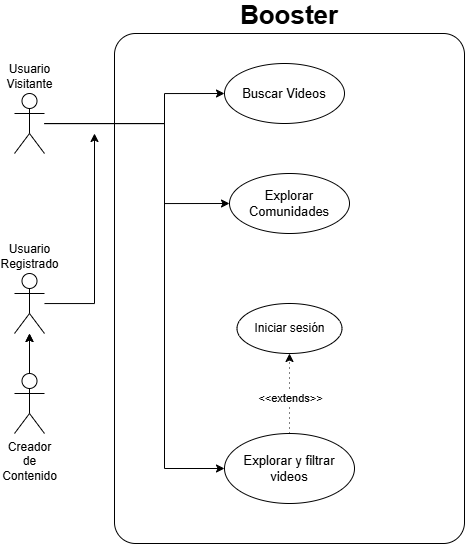
\includegraphics[width=0.8\textwidth]{casos-uso/exploracion-busqueda.png}
  \caption{Exploración y búsqueda de contenido - Casos de uso}
\end{figure}

\textbf{Descripción}


%BUSCAR VIDEOS

\begin{longtable}{|p{0.28\textwidth}|p{0.64\textwidth}|}
\hline
\rowcolor[gray]{0.75}
\multicolumn{2}{|c|}{\textbf{Caso de uso: Buscar videos}} \\
\hline
\textbf{Actores} & Usuario visitante, Usuario registrado \\
\hline
\textbf{Descripción} & Permite al usuario buscar videos en la plataforma a partir de su título, descripción o creador. La búsqueda puede apoyarse también en mecanismos de búsqueda semántica. \\
\hline
\textbf{Precondiciones} & El usuario accede a la interfaz de búsqueda de la plataforma. \\
\hline
\textbf{Curso principal} &
\begin{enumerate}
    \item El usuario accede a la barra o sección de búsqueda.
    \item El sistema solicita el término de búsqueda.
    \item El usuario introduce una consulta.
    \item El sistema procesa la consulta.
    \item El sistema busca videos por título, descripción o creador.
    \item El sistema muestra la lista de resultados encontrados.
    \item El usuario selecciona uno de los resultados para acceder al contenido.
\end{enumerate} \\
\hline


\rowcolor[gray]{0.75}
\multicolumn{2}{|c|}{\textbf{Curso alternativo al paso 5: sin resultados}} \\
\hline
\multicolumn{2}{|p{0.92\textwidth}|}{
\begin{enumerate}[label=5\alph*.]
    \item Si no se encuentran videos coincidentes, el sistema informa de que no existen resultados para la consulta realizada.
    \item El sistema invita al usuario a realizar otra búsqueda.
\end{enumerate}
} \\
\hline

\textbf{Postcondiciones} & El usuario obtiene una lista de videos o creadores de contenido relacionados con la consulta introducida. \\
\hline
\textbf{Requisitos relacionados} & RF-EB 1 \\
\hline
\end{longtable}

%EXPLORAR Y FILTRAR


\begin{longtable}{|p{0.28\textwidth}|p{0.64\textwidth}|}
\hline
\rowcolor[gray]{0.75}
\multicolumn{2}{|c|}{\textbf{Caso de uso: Explorar y filtrar videos}} \\
\hline
\textbf{Actores} & Usuario visitante, Usuario registrado \\
\hline
\textbf{Descripción} & Permite al usuario explorar la cuadrícula principal de videos recomendados y aplicar filtros sobre el contenido disponible, por ejemplo por categoría, contenido generado por inteligencia artificial o formato vertical. Además, permite explorar los videos más recientes de las comunidades y canales que sigue \\
\hline
\textbf{Precondiciones} & El usuario accede a la pantalla principal o a la sección de exploración de videos. \\
\hline
\textbf{Curso principal} &
\begin{enumerate}
    \item El usuario accede a la sección principal de exploración de videos.
    \item El sistema muestra una cuadrícula de videos recomendados.
    \item El usuario accede a las opciones de filtrado.
    \item El usuario selecciona uno o varios filtros, como categoría, contenido hecho por inteligencia artificial o formato vertical.
    \item El sistema aplica los filtros seleccionados.
    \item El sistema actualiza la cuadrícula de videos mostrada.
    \item El usuario explora los resultados filtrados y selecciona un video si lo desea.
    \item El usuario accede a la pestaña de comunidades.
    \item El sistema le muestra los videos más recientes de las comunidades que sigue.
    \item El usuario accede a la pestaña de canales.
    \item El sistema muestra los videos más recientes de los canales que sigue. 
    
\end{enumerate} \\
\hline

\rowcolor[gray]{0.75}
\multicolumn{2}{|c|}{\textbf{Curso alternativo al paso 2: error al cargar recomendaciones}} \\
\hline
\multicolumn{2}{|p{0.92\textwidth}|}{
\begin{enumerate}[label=2\alph*.]
    \item Si no es posible cargar la cuadrícula principal de recomendaciones, el sistema muestra un mensaje de error.
    \item El sistema permite reintentar la carga.
\end{enumerate}
} \\
\hline

\rowcolor[gray]{0.75}
\multicolumn{2}{|c|}{\textbf{Curso alternativo al paso 4: filtros sin resultados}} \\
\hline
\multicolumn{2}{|p{0.92\textwidth}|}{
\begin{enumerate}[label=4\alph*.]
    \item Si la combinación de filtros seleccionada no produce resultados, el sistema lo informa.
\end{enumerate}
} \\
\hline


\rowcolor[gray]{0.75}
\multicolumn{2}{|c|}{\textbf{Curso alternativo a los pasos 8 y 10: usuario sin sesión}} \\
\hline
\multicolumn{2}{|p{0.92\textwidth}|}{
\begin{enumerate}[label=\roman*.]
    \item El usuario no puede acceder a las secciones que requieren autenticación.
    \item El sistema muestra un mensaje solicitando al usuario que inicie sesión para acceder a estas pestañas.
\end{enumerate}
} \\
\hline


\textbf{Postcondiciones} & El usuario visualiza una cuadrícula de videos adaptada a los filtros seleccionados. \\
\hline
\textbf{Requisitos relacionados} & RF-EB 2, RF-EB 3, RF-EB 4,  RF-EB 5 \\
\hline
\end{longtable}


%EXPLORAR COMUNIDADES
\begin{longtable}{|p{0.28\textwidth}|p{0.64\textwidth}|}
\hline
\rowcolor[gray]{0.75}
\multicolumn{2}{|c|}{\textbf{Caso de uso: Explorar comunidades}} \\
\hline
\textbf{Actores} & Usuario visitante, Usuario registrado \\
\hline
\textbf{Descripción} & Permite al usuario explorar comunidades en la plataforma y ver el contenido reciente de estas. \\
\hline
\textbf{Precondiciones} & El usuario accede a la sección de exploración de comunidades. \\
\hline
\textbf{Curso principal} &
\begin{enumerate}
    \item El usuario accede a la sección de exploración de comunidades.
    \item El sistema muestra comunidades destacados o recientes.
    \item El usuario navega entre las opciones disponibles.
    \item El usuario selecciona una comunidad o canal para consultar su contenido.
    \item El sistema muestra la información y el contenido asociado a la comunidad o canal seleccionado.
\end{enumerate} \\
\hline


\rowcolor[gray]{0.75}
\multicolumn{2}{|c|}{\textbf{Curso alternativo al paso 2: sin contenido disponible}} \\
\hline
\multicolumn{2}{|p{0.92\textwidth}|}{
\begin{enumerate}[label=2\alph*.]
    \item Si no existen comunidades o canales disponibles para mostrar, el sistema informa de ello.
    \item El sistema mantiene la sección accesible para futuras consultas.
\end{enumerate}
} \\
\hline

\textbf{Postcondiciones} & El usuario visualiza comunidades, y accede a su contenido reciente. \\
\hline
\textbf{Requisitos relacionados} & RF-EB 6 \\
\hline
\end{longtable}



\subsection{Interacción social}

Los casos de uso identificados relacionados con la interacción social son:

\begin{enumerate}
    \item Calificar video
    \item Gestión de comentarios
    \item Donar puntos de experiencia
\end{enumerate}

\clearpage

\textbf{Diagrama}

\begin{figure}[H]
  \centering
  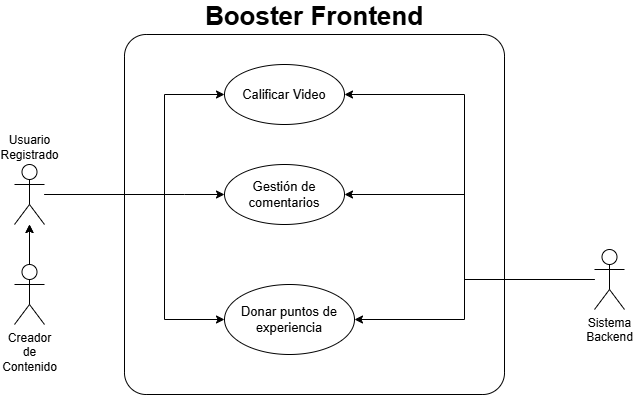
\includegraphics[width=1\textwidth]{casos-uso/interaccion-social.png}
  \caption{Interacciones en la plataforma  - Casos de uso}
\end{figure}


\textbf{Descripción}

Gestión de comentarios incluye comentar, responder, editar, eliminar, mostrarlos y recomendar. 

\subsection{Comunidades}

\begin{enumerate}
    \item Interactuar con comunidades
    \item Consultar comunidades
    \item Buscar y filtrar comunidades
\end{enumerate}

\textbf{Diagrama}

\begin{figure}[H]
  \centering
  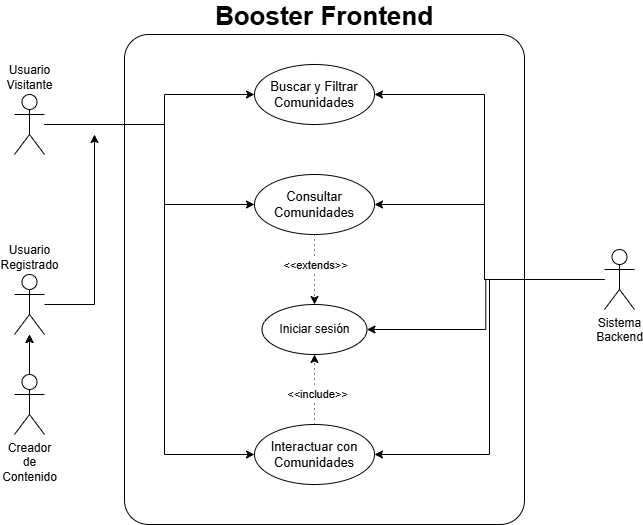
\includegraphics[width=1\textwidth]{casos-uso/comunidades.png}
  \caption{Comunidades  - Casos de uso}
\end{figure}


\textbf{Descripción}

 Interactuar con comunidades incluye crear, unirse, abandonar.
 Consultar es: ver videos de las comnuidades, ver comunidades a las que pertenece
 EXplorar comunidades tiene buscar por nombre,descripcion y filtrar.  

\subsection{Canales}

\begin{enumerate}
    \item Gestionar canal
    \item Consultar canal y canales seguidos
    \item Interactuar con canales
\end{enumerate}

\textbf{Diagrama}
\begin{figure}[H]
  \centering
  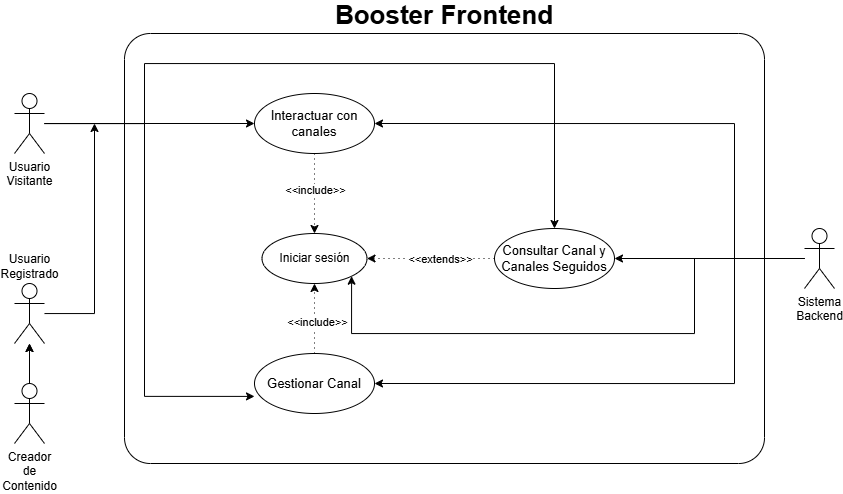
\includegraphics[width=1\textwidth]{casos-uso/canales.png}
  \caption{Canales - Casos de uso}
\end{figure}

\textbf{Descripción}

Consultar canal incluye consultar a los que sigue: extends de login
\subsection{Gamificación}

\begin{enumerate}
    \item Ganar puntos de experiencia
    \item Consultar puntos de boost y nivel de canal
    \item Consultar rankings
    \item Consultar tienda de recompensas
    \item Comprar artículos de personalización
    \item Equipar y consultar artículos de personalización
\end{enumerate}

\textbf{Diagrama}
\begin{figure}[H]
  \centering
  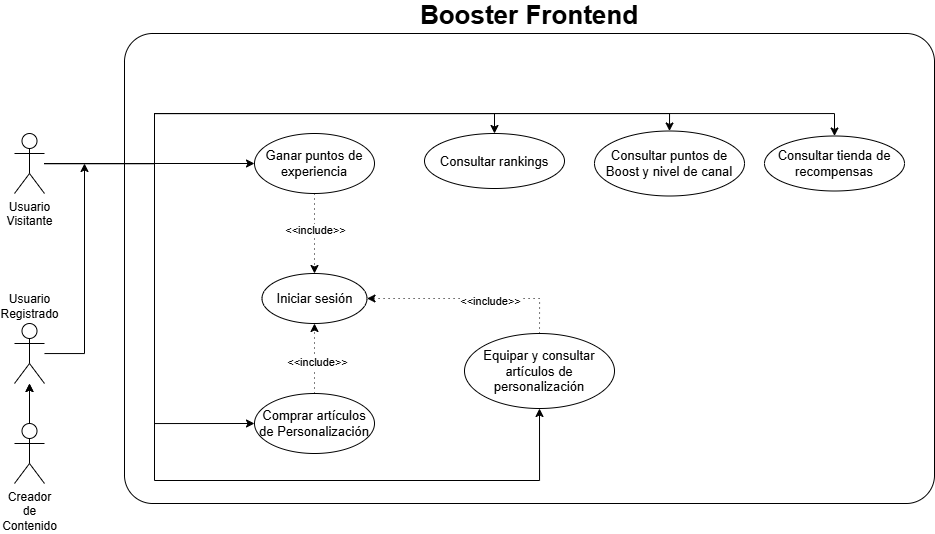
\includegraphics[width=1\textwidth]{casos-uso/gamificacion.png}
  \caption{Gamificación- Casos de uso}
\end{figure}


\textbf{Descripción}


\subsection{Diagramas de casos de uso}

\subsubsection{Gestión de usuarios}








\subsubsection{Carga y gestión de videos}


\subsection{Reproducción y consumo de contenido}


\subsection{Descripción de casos de uso}





\section{Diagramas de secuencia}

En esta sección se recopilan algunos de los diagramas de secuencia más importantes en la aplicación final. 

\section{Diagrama Entidad Relación}

